%%%%%%%%%%%%%%%%%%%%%%%%%%%%%%%%%%%%%%%%%%%%%%%%%%%%%%%%%%%%%%%%%%%%
\section{Organization and Management}
\label{sec:fdsp-apa-org}

Coordination of the groups participating in the \dword{dune} \dword{apa} Consortium is critical to successfully executing the large-scale multi-year construction project that is needed to produce high-quality \dword{apa}s for the \dword{dune} \dwords{spmod}.   The \dword{apa} consortium comprises \num{21} institutions, of which \num{14} are in the USA and \num{7} in the UK (see Table~\ref{tab:apa-institutions}). The consortium is organized along the main deliverables, which are the final design of the \dword{apa} and the \dword{apa} production and installation procedures (see Figure~\ref{fig:apa-consortium-structure}).  The two main centers of \dword{apa} construction are in the USA and the UK, so usually the leaders of a working group are chosen to represent the main stakeholders to ensure that common procedures and tooling are developed.  We plan to produce half of the \dword{dune} \dwords{apa}s in the USA and half in the UK.

\begin{dunefigure}[APA consortium organizational chart]{fig:apa-consortium-structure}
{\dword{apa} consortium organizational chart.}
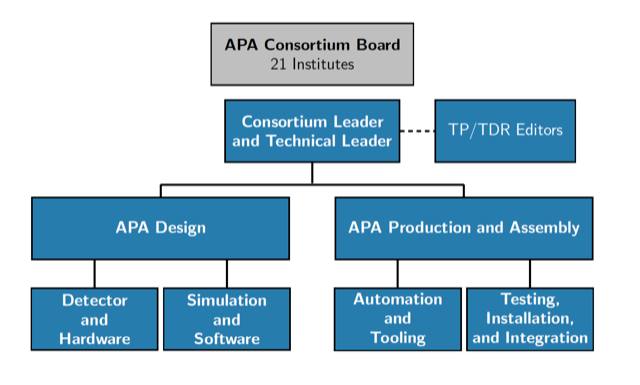
\includegraphics[width=0.7\textwidth,trim=0mm 0mm 0mm 0mm,clip]{apa-consortium-orgchart-nonames}
%\includegraphics[width=0.80\textwidth]{apa-consortium-structure-new.png}  %updated org chart for consistency - Ddm
\end{dunefigure}
%
\begin{dunetable}
[APA consortium institutions]
{ll}
{tab:apa-institutions}
{Current APA consortium institutions and countries.}
Institution & \bfseries{Country} \\ \toprowrule
University of Cambridge     &  UK       \\ \colhline
Daresbury Laboratory - Science and Technology Facilities Council & UK \\ \colhline
Lancaster University & UK \\ \colhline
University of Liverpool & UK \\ \colhline
University of Manchester & UK \\ \colhline
University of Sheffield & UK \\ \colhline
University of Sussex & UK \\ \colhline
%Argonne National Laboratory & USA \\ \colhline
Brookhaven National Laboratory & USA \\ \colhline
University of Chicago & USA \\ \colhline
Colorado State University & USA \\ \colhline
Harvard University & USA \\ \colhline
University of Houston & USA \\ \colhline
University of Iowa & USA \\ \colhline
University of Mississippi & USA \\ \colhline
Northern Illinois University & USA \\ \colhline
%South Dakota School of Mines and Technology & USA \\ \colhline
Syracuse University & USA \\ \colhline
University of Texas at Arlington & USA \\ \colhline
Tufts University & USA \\ \colhline
College of William \& Mary & USA \\ \colhline
University of Wisconsin-Madison, Physical Sciences Laboratory & USA \\ \colhline
Yale University & USA \\
\end{dunetable}



%%%%%%%%%%%%%%%%%%%%%%%%%%%%%%%%%%%%%%
%\subsection{Planning Assumptions}
%\label{sec:fdsp-apa-org-assmp}

%The planning assumes nine \dword{apa} assembly lines at different locations in the UK and the USA.  We assume set up time for the factories will take about one year. It will take approximately \num{40} shifts (8 hours) of clock time  to construct a single \dword{apa}. Assuming an 8 hours shift/day, we can construct the \num{150} \dwords{apa} required for one \dword{spmod} %\SI{10}{kton} module within about two and a half years.

%%%%%%%%%%%%%%%%%%%%%%%%%%%%%%%%%%%%%%
%\subsection{WBS and Responsibilities}
%\label{sec:fdsp-apa-org-wbs}

%Here, we only discuss the top-level WBS elements: (1)~design, engineering and prototypes, (2)~production setup, (3)~production, (4)~integration and installation.

The university groups and \dword{bnl} are responsible for validating  the design, while engineering and the production set up is being developed at PSL %at the University of Wisconsin-Madison 
(USA) and Daresbury Laboratory (UK), where the \dwords{apa} for \dword{pdsp} have been built. 
%with contributions from university groups. \fixme{Nora: I think what you mean here is that the university groups will contribute to developing the engineering and production set up. To make that clear, you likely will need another sentence instead of "with contributions from university groups". So "The university groups will contribute to developing..."} 
In addition to PSL and Daresbury Laboratory, the University of Chicago and Yale University are developing detailed plans for the layouts, activities, and schedule at each site. 
%The production sites will require significant help from university groups during the production process. 

In addition to the \dword{apa} production sites, a successful production effort will require significant and sustained contributions from university groups throughout the production process.  Table~\ref{tab:apa-institution-roles} and Figure~\ref{fig:apa-construction-org} list the main work packages that are part of the overall \dword{apa} construction process and the institutions in the USA and UK who are taking the leading roles in each effort.  The tasks range from the production of bare support frames, to the assembly and testing of many thousands of wire boards, to the procurement of the custom transport crates for shipping the completed \dword{apa}s.  The on-time supply of materials to each of the \dword{apa} production sites will be imperative to maintaining the production schedule, and detailed plans are being developed for the execution of the project in both countries. 

%In addition to a project management team to oversee operations across the project, all work packages have an identified faculty lead. 

%The steel for the frames most likely will be bought from a single vendor but will be assembled in the USA and the UK separately. We are still exploring the option to assemble the frames in house or in collaboration with industrial partners. Other significant components include on-\dword{apa} electronics boards. Design modifications for \dword{pdsp} are the responsibility of PSL, University of Wisconsin-Madison. The boards will be produced by industry partners, but the testing will be distributed among consortium institutions. The shipping of the \dwords{apa} is the responsibility of the production factories in the USA and the UK, while the design of the \dword{apa} transport frame is responsibility of the UK groups. The integration and installation are a joint responsibility of the consortium, with UK taking a leading role for integration and US for installation. Argonne National Laboratory (ANL) is cooperating with the technical coordination group for the design of the \dword{apa} support system within the cryostat.

\begin{dunefigure}[APA construction organizational chart]{fig:apa-construction-org}
{\dword{apa} construction project organizational.}
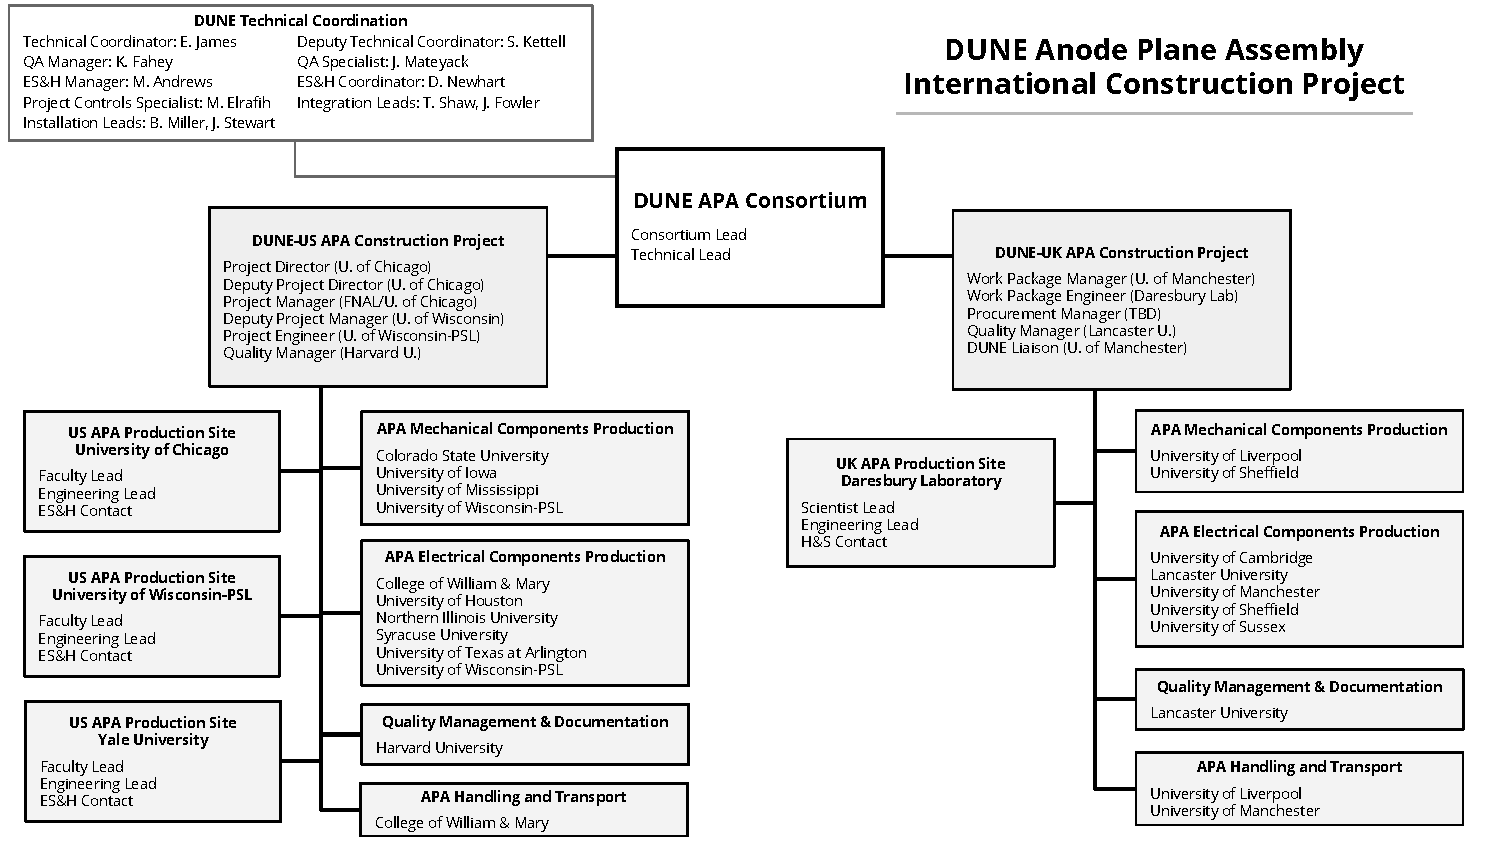
\includegraphics[width=1\textwidth,trim=0mm 0mm 0mm 0mm,clip]{graphics/sp-apa-construction-org-chart.pdf}
%\includegraphics[width=0.80\textwidth]{apa-consortium-structure-new.png}  %updated org chart for consistency - Ddm
\end{dunefigure}

\begin{dunetable}
[APA production institutional responsibilities]
{ll}
{tab:apa-institution-roles}
{Institutional responsibilities for \dword{apa} production in the UK and USA.}
APA Construction Work Packages & \multicolumn{1}{c}{\bfseries{Institutions}} \\ \toprowrule
\rowcolor{lightgray} \multicolumn{2}{c}{Production in the UK} \\ \colhline
APA production site  &  Daresbury Laboratory \\ \colhline
$U/V$-plane wire boards & University of Cambridge, University of Sussex \\ \colhline
$X/G$-plane wire boards & Lancaster University, University of Sheffield \\ \colhline
G-bias boards & University of Manchester \\ \colhline
CR boards & University of Manchester \\ \colhline
Cold electronics adapter boards & University of Sheffield \\ \colhline
Grounding mesh frames & University of Sheffield \\ \colhline
APA frames & University of Liverpool \\ \colhline
APA transport crates & University of Liverpool, University of Manchester \\ \colhline
Yokes and structural tees & University of Liverpool  \\ \colhline
QA/QC management & Lancaster University \\ \colhline
\rowcolor{lightgray} \multicolumn{2}{c}{Production in the US} \\ \colhline
APA production site & University of Wisconsin-PSL \\ \colhline
APA production site & University of Chicago  \\ \colhline
APA production site & Yale University  \\ \colhline 
U/V-plane wire boards & College of William \& Mary  \\ \colhline
X-plane wire boards & University of Texas at Arlington  \\ \colhline
G-plane wire boards & University of Houston  \\ \colhline
G-bias boards & Syracuse University  \\ \colhline
CR boards & University of Wisconsin-PSL \\ \colhline
Cold electronics adapter boards & Northern Illinois University  \\ \colhline
Grounding mesh frames & University of Chicago  \\ \colhline
APA frames & University of Iowa, University of Wisconsin-PSL \\ \colhline
APA transport crates & College of William \& Mary  \\ \colhline
Yokes and structural tees & University of Wisconsin-PSL  \\ \colhline
\dword{ce} interface hardware & Colorado State University, University of Wisconsin-PSL  \\ \colhline
QA/QC management, wire tension & Harvard University  \\ 
%Construction support software & Otterbein University  \\ \Xhline{3\arrayrulewidth}
\end{dunetable}